\chapter{Thực nghiệm và đánh giá}
\label{ch:experiment}

Chương này trình bày thiết lập thực nghiệm, kết quả đánh giá và phân tích hệ thống phát hiện ESG-washing đã đề xuất ở Chương~\ref{ch:method}. Mục~\ref{sec:research_questions} phát biểu lại các câu hỏi nghiên cứu. Mục~\ref{sec:exp_setup} mô tả dữ liệu, môi trường huấn luyện và cấu hình siêu tham số. Các mục từ~\ref{sec:topic_results} đến~\ref{sec:ewri_results} lần lượt báo cáo kết quả từng giai đoạn pipeline. Mục~\ref{sec:qualitative} thực hiện phân tích định tính, và Mục~\ref{sec:discussion} thảo luận ý nghĩa cùng hạn chế.


%% ============================================================
%% 4.1 CÂU HỎI NGHIÊN CỨU
%% ============================================================
\section{Câu hỏi nghiên cứu}
\label{sec:research_questions}

Khóa luận đặt ra ba câu hỏi nghiên cứu chính:

\begin{description}
    \item[\textbf{RQ1}] \textit{Phương pháp neuro-symbolic kết hợp PhoBERT và các quy tắc ký hiệu miền ESG có hiệu quả như thế nào trong bài toán phân loại chủ đề ESG và mức độ hành động trên báo cáo thường niên ngân hàng Việt Nam?}
    \item[\textbf{RQ2}] \textit{Phương pháp liên kết bằng chứng ngữ nghĩa hai giai đoạn (semantic retrieval + NLI verification) có cải thiện chất lượng đánh giá mức độ thực chất của các tuyên bố ESG so với phương pháp dựa trên cửa sổ ngữ cảnh?}
    \item[\textbf{RQ3}] \textit{Chỉ số EWRI phản ánh mức độ rủi ro ESG-washing như thế nào, và có sự khác biệt đáng kể giữa các ngân hàng cùng xu hướng minh bạch trong giai đoạn 2020--2024?}
\end{description}


%% ============================================================
%% 4.2 DỮ LIỆU VÀ THIẾT LẬP THỰC NGHIỆM
%% ============================================================
\section{Dữ liệu và thiết lập thực nghiệm}
\label{sec:exp_setup}

\subsection{Tập dữ liệu}
\label{subsec:dataset}

Tập dữ liệu được xây dựng từ báo cáo thường niên của 10 ngân hàng thương mại Việt Nam trong giai đoạn 2020--2024, tổng cộng 50 quan sát ngân hàng-năm (chi tiết quy trình thu thập và tiền xử lý xem Mục~\ref{sec:data_preparation}). Sau khi phân đoạn và lọc, corpus gồm 114.865 câu, trong đó 32.260 câu được phân loại thuộc nhóm ESG (khác Non\_ESG).

Dữ liệu huấn luyện cho hai bộ phân loại được chia theo tỉ lệ 80/10/10 với phân tầng theo nhãn (stratified split). Bảng~\ref{tab:data_split} tóm tắt quy mô các tập.

\begin{table}[H]
\centering
\caption{Quy mô tập dữ liệu huấn luyện, xác thực và kiểm thử.}
\label{tab:data_split}
\begin{tabular}{lrrr}
\toprule
\textbf{Bộ phân loại} & \textbf{Train} & \textbf{Val} & \textbf{Test} \\
\midrule
Chủ đề ESG (6 nhãn)        & 91.188 & 11.399 & 11.399 \\
Mức độ hành động (3 nhãn)   & 25.808 &  3.226 &  3.226 \\
\bottomrule
\end{tabular}
\end{table}

Phân phối nhãn của tập huấn luyện được trình bày trong Bảng~\ref{tab:label_dist}. Tập dữ liệu chủ đề có sự mất cân bằng rõ rệt: nhãn Non\_ESG chiếm 71,7\% tổng số mẫu, trong khi S\_community chỉ chiếm 1,8\%. Tương tự, tập dữ liệu hành động có nhãn Indeterminate chiếm 64,9\% và Planning chỉ 2,8\%. Để xử lý mất cân bằng, hệ thống sử dụng trọng số lớp theo phương pháp \textit{sqrt-inverse} (Mục~\ref{sec:training}).

\begin{table}[H]
\centering
\caption{Phân phối nhãn trong tập huấn luyện.}
\label{tab:label_dist}
\begin{tabular}{lrr|lrr}
\toprule
\multicolumn{3}{c|}{\textbf{Chủ đề ESG}} & \multicolumn{3}{c}{\textbf{Mức độ hành động}} \\
\textbf{Nhãn} & \textbf{Số mẫu} & \textbf{\%} & \textbf{Nhãn} & \textbf{Số mẫu} & \textbf{\%} \\
\midrule
Non\_ESG      & 65.338 & 71,7 & Indeterminate & 16.756 & 64,9 \\
G             & 13.450 & 14,8 & Implemented   &  8.322 & 32,2 \\
S\_labor      &  4.470 &  4,9 & Planning      &    730 &  2,8 \\
S\_product    &  3.904 &  4,3 &               &        &      \\
E             &  2.429 &  2,7 &               &        &      \\
S\_community  &  1.597 &  1,8 &               &        &      \\
\bottomrule
\end{tabular}
\end{table}


\subsection{Môi trường huấn luyện}
\label{subsec:training_env}

Toàn bộ quá trình huấn luyện được thực hiện trên nền tảng Kaggle với GPU Tesla P100 (16\,GB VRAM), RAM 30\,GB, và lưu trữ 73\,GB. Thời gian huấn luyện mỗi cấu hình khoảng 2--2,5 giờ cho bộ phân loại chủ đề (5 epoch $\times$ 14.250 bước) và 36--42 phút cho bộ phân loại hành động (5 epoch $\times$ 4.035 bước). Pipeline suy luận (inference) trên toàn bộ 50 báo cáo hoàn thành trong khoảng 45 phút trên cùng cấu hình.


\subsection{Cấu hình siêu tham số}
\label{subsec:hyperparams}

Bảng~\ref{tab:hyperparams} tổng hợp các siêu tham số chính cho cả hai bộ phân loại. Mô hình nền tảng (backbone) là PhoBERT-base \citep{nguyen2020phobert} với 135 triệu tham số, được tinh chỉnh toàn bộ (full fine-tuning). Cấu hình neuro-symbolic sử dụng trọng số ràng buộc $\lambda = 0{,}3$ cho hàm mất mát ngữ nghĩa và lưới tìm kiếm $\alpha \in \{0{,}3;\ 0{,}5;\ 0{,}7;\ 0{,}9\}$ cho suy luận có ràng buộc (constrained inference).

\begin{table}[H]
\centering
\caption{Cấu hình siêu tham số huấn luyện.}
\label{tab:hyperparams}
\begin{tabular}{ll}
\toprule
\textbf{Tham số} & \textbf{Giá trị} \\
\midrule
Mô hình nền tảng     & PhoBERT-base (135M params) \\
Độ dài tối đa (token) & 128 \\
Số epoch              & 5 \\
Batch size (train/eval) & 16 / 32 \\
Learning rate         & $2 \times 10^{-5}$ \\
Weight decay          & 0,01 \\
Warmup ratio          & 10\% \\
LR scheduler          & Linear decay \\
Trọng số lớp          & sqrt-inverse \\
Max gradient norm     & 1,0 \\
Early stopping patience & 2 epoch \\
Seed                   & 42 \\
\midrule
\multicolumn{2}{l}{\textit{Neuro-symbolic}} \\
$\lambda$ (constraint loss)    & 0,3 \\
$w_{\text{exactly\_one}}$      & 1,0 \\
$w_{\text{implication}}$       & 0,5 \\
$w_{\text{negation}}$          & 0,5 \\
$\alpha$ grid (inference)      & \{0,3; 0,5; 0,7; 0,9\} \\
Min confidence                 & 0,3 \\
\bottomrule
\end{tabular}
\end{table}


\subsection{Độ đo đánh giá}
\label{subsec:metrics}

Các độ đo được sử dụng xuyên suốt thực nghiệm bao gồm:

\begin{itemize}
    \item \textbf{Macro F1}: Trung bình cộng F1 của tất cả các lớp, mỗi lớp có trọng số bằng nhau bất kể kích thước. Đây là độ đo chính (\texttt{metric\_for\_best\_model}) do tập dữ liệu mất cân bằng nghiêm trọng.
    \item \textbf{Micro F1}: F1 tính trên tổng TP, FP, FN toàn cục, phản ánh hiệu suất trên các lớp phổ biến.
    \item \textbf{Rule coverage}: Tỉ lệ mẫu có ít nhất một ràng buộc ký hiệu được kích hoạt (chỉ áp dụng cho cấu hình neuro-symbolic).
    \item \textbf{Hệ số tương quan Spearman} ($\rho$): Đo mối liên hệ đơn điệu giữa các biến EWRI, dùng cho phân tích tương quan cấp ngân hàng-năm.
    \item \textbf{Eta-squared} ($\eta^2$): Kích thước hiệu ứng của biến phân loại (nhãn hành động) lên biến liên tục (washing risk score).
\end{itemize}


%% ============================================================
%% 4.3 KẾT QUẢ PHÂN LOẠI CHỦ ĐỀ ESG (RQ1)
%% ============================================================
\section{Kết quả phân loại chủ đề ESG}
\label{sec:topic_results}

\subsection{So sánh Baseline và Neuro-Symbolic}
\label{subsec:topic_baseline_vs_neuro}

Bảng~\ref{tab:topic_val} trình bày kết quả trên tập xác thực (validation) qua 5 epoch huấn luyện, so sánh hai cấu hình: \textit{Baseline} (PhoBERT fine-tuning thuần) và \textit{Neuro-Symbolic} (PhoBERT + Semantic Loss).

\begin{table}[H]
\centering
\caption{Kết quả phân loại chủ đề ESG trên tập xác thực (validation). \textit{Baseline}: PhoBERT fine-tuning; \textit{Neuro}: PhoBERT + semantic loss ($\lambda = 0{,}3$).}
\label{tab:topic_val}
\begin{tabular}{c|cc|cc}
\toprule
 & \multicolumn{2}{c|}{\textbf{Baseline}} & \multicolumn{2}{c}{\textbf{Neuro-Symbolic}} \\
\textbf{Epoch} & \textbf{Macro F1} & \textbf{Micro F1} & \textbf{Macro F1} & \textbf{Micro F1} \\
\midrule
1 & 0,7742 & 0,8647 & 0,7635 & 0,8522 \\
2 & 0,8107 & 0,8939 & 0,8035 & 0,8920 \\
3 & 0,8211 & 0,9024 & 0,8065 & 0,8953 \\
4 & 0,8226 & 0,9057 & 0,8245 & 0,9081 \\
5 & 0,8308 & 0,9093 & 0,8271 & 0,9085 \\
\bottomrule
\end{tabular}
\end{table}

Cấu hình Baseline đạt Macro F1 = 0,8308 và Micro F1 = 0,9093 ở epoch cuối, cao hơn nhẹ so với Neuro-Symbolic (Macro F1 = 0,8271, Micro F1 = 0,9085). Tuy nhiên, sự khác biệt này chỉ ở mức 0,4 điểm phần trăm --- không có ý nghĩa thống kê khi xét khoảng tin cậy từ một lần huấn luyện duy nhất.

Điều đáng chú ý là cấu hình Neuro-Symbolic có training loss thấp hơn ổn định (0,317 ở epoch 5 so với 0,214 của Baseline), cho thấy Semantic Loss bổ sung tín hiệu regularization hiệu quả, tránh hiện tượng overfitting. Thời gian huấn luyện tăng khoảng 19\% (2 giờ 28 phút so với 2 giờ 05 phút) do chi phí tính toán ràng buộc ký hiệu trên mỗi batch.

\subsection{Suy luận có ràng buộc (Constrained Inference)}
\label{subsec:topic_constrained}

Sau khi huấn luyện, hệ thống áp dụng \textit{constrained inference} trên tập xác thực với lưới tìm kiếm $\alpha \in \{0{,}3;\ 0{,}5;\ 0{,}7;\ 0{,}9\}$. Kỹ thuật này điều chỉnh logit đầu ra bằng cách cộng thêm tín hiệu từ các quy tắc ký hiệu (Mục~\ref{sec:training}), cho phép tri thức miền ảnh hưởng đến quyết định phân loại mà không thay đổi mô hình. Giá trị $\alpha$ tối ưu được chọn là giá trị cho Macro F1 cao nhất trên tập xác thực.

Đường cong huấn luyện (Hình~\ref{fig:training_curves}, trái) cho thấy cả hai cấu hình hội tụ tốt sau 5 epoch, với xu hướng cải thiện bền vững qua các epoch, không có dấu hiệu suy giảm hiệu suất.

\begin{figure}[H]
    \centering
    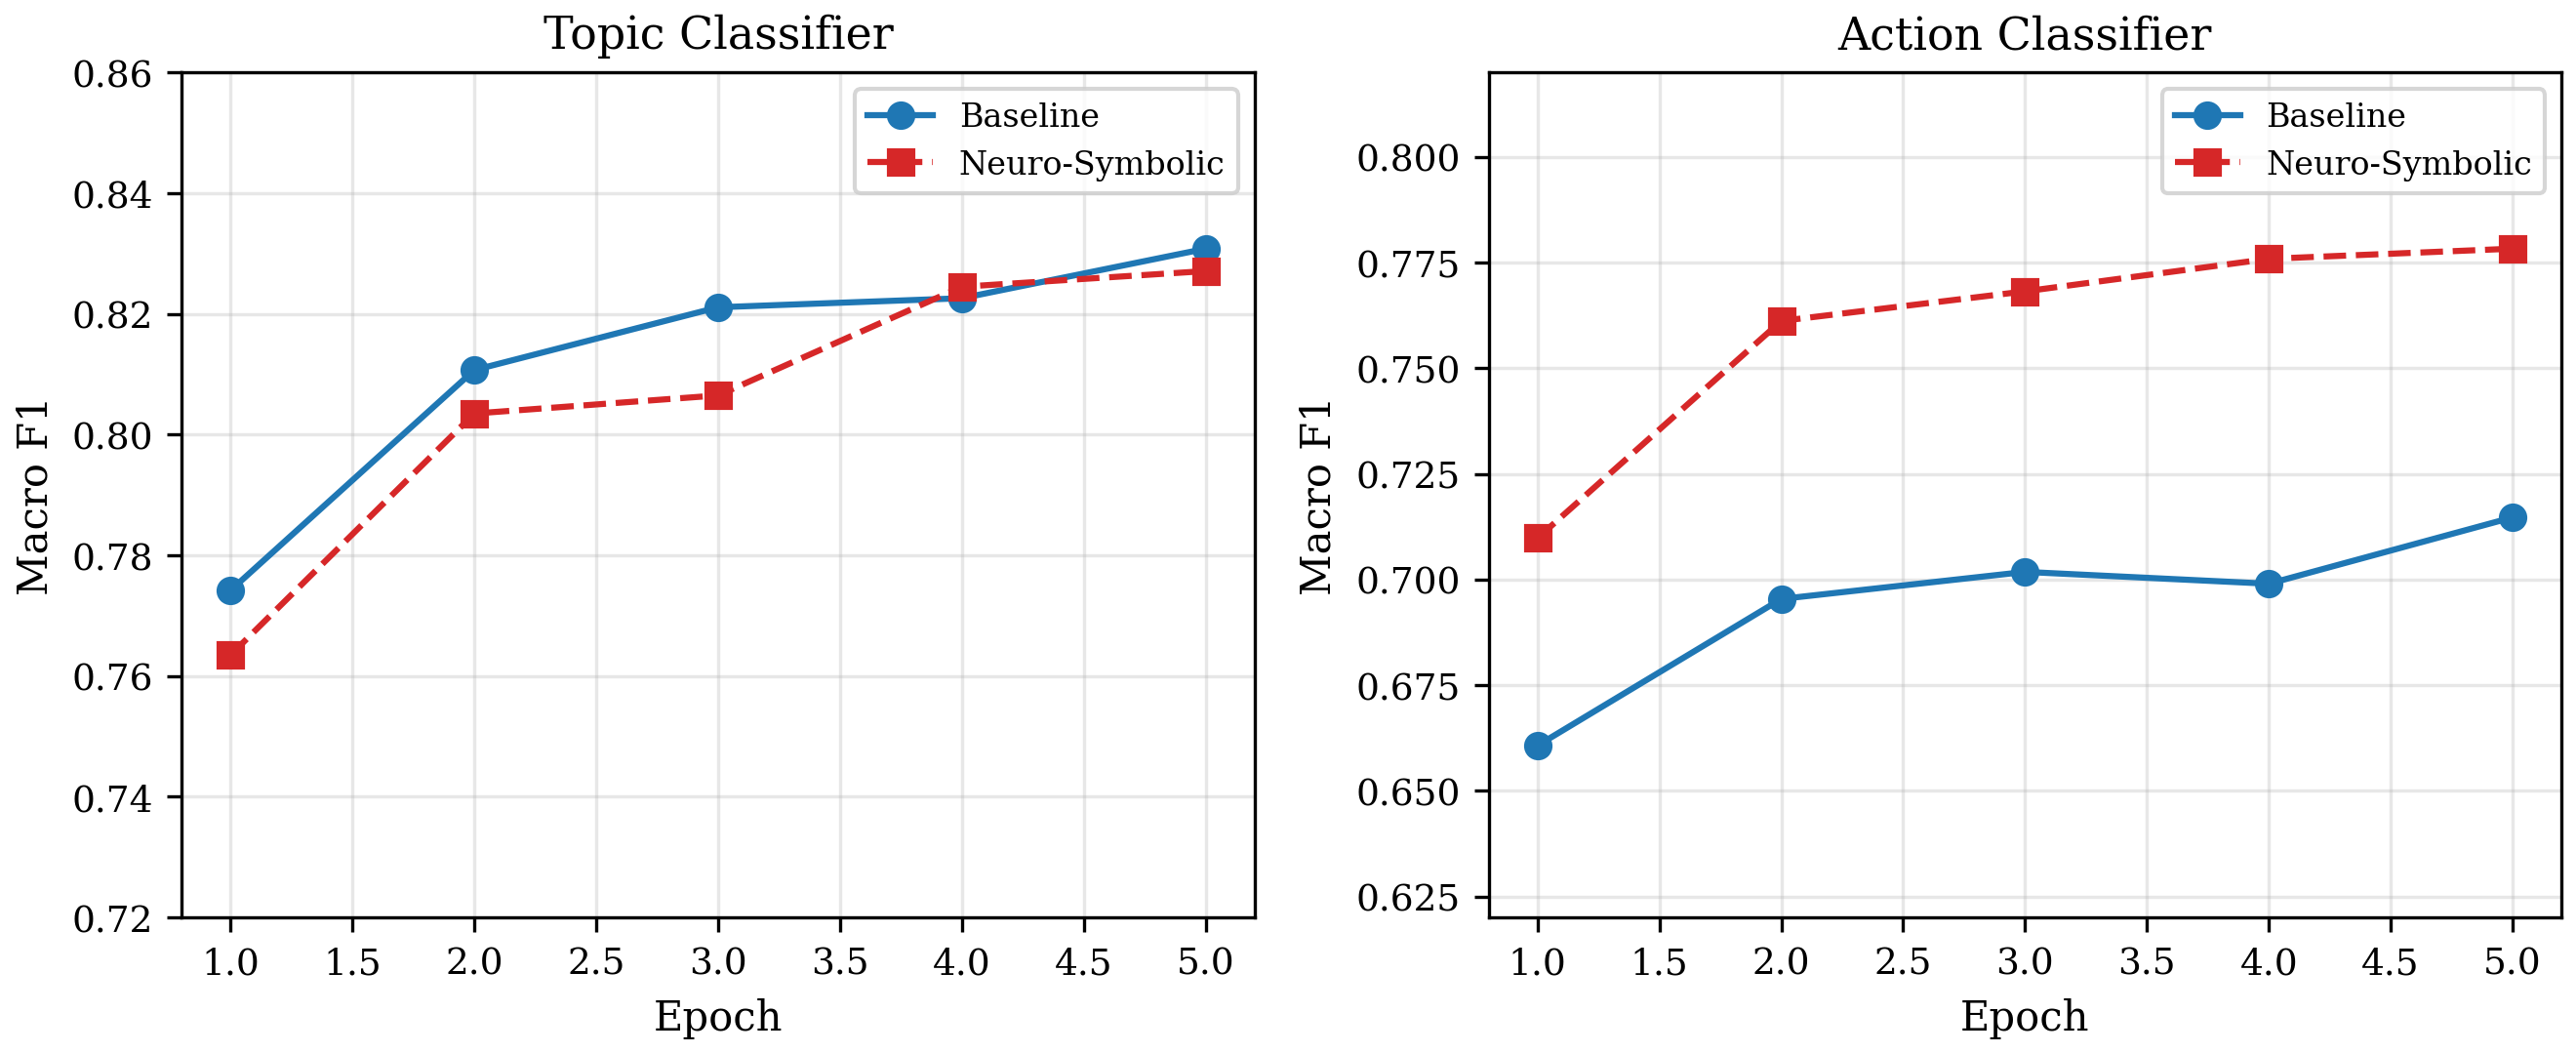
\includegraphics[width=0.9\textwidth]{figures/training_curves.png}
    \caption{Đường cong Macro F1 trên tập xác thực qua 5 epoch huấn luyện. Trái: bộ phân loại chủ đề ESG (6 nhãn); Phải: bộ phân loại mức độ hành động (3 nhãn). Đường liền: Baseline; Đường đứt: Neuro-Symbolic.}
    \label{fig:training_curves}
\end{figure}


%% ============================================================
%% 4.4 KẾT QUẢ PHÂN LOẠI MỨC ĐỘ HÀNH ĐỘNG (RQ1)
%% ============================================================
\section{Kết quả phân loại mức độ hành động}
\label{sec:action_results}

\subsection{So sánh Baseline và Neuro-Symbolic}
\label{subsec:action_baseline_vs_neuro}

Bảng~\ref{tab:action_val} trình bày kết quả bộ phân loại mức độ hành động trên tập xác thực. Khác với bộ phân loại chủ đề, cấu hình Neuro-Symbolic cho kết quả \textit{vượt trội rõ rệt} so với Baseline.

\begin{table}[H]
\centering
\caption{Kết quả phân loại mức độ hành động trên tập xác thực. Neuro-Symbolic vượt trội Baseline ở mọi epoch.}
\label{tab:action_val}
\begin{tabular}{c|cc|cc}
\toprule
 & \multicolumn{2}{c|}{\textbf{Baseline}} & \multicolumn{2}{c}{\textbf{Neuro-Symbolic}} \\
\textbf{Epoch} & \textbf{Macro F1} & \textbf{Micro F1} & \textbf{Macro F1} & \textbf{Micro F1} \\
\midrule
1 & 0,6607 & 0,7823 & 0,7098 & 0,8342 \\
2 & 0,6954 & 0,8129 & 0,7612 & 0,8763 \\
3 & 0,7018 & 0,8138 & 0,7682 & 0,8819 \\
4 & 0,6990 & 0,8100 & 0,7759 & 0,8881 \\
5 & 0,7147 & 0,8275 & 0,7783 & 0,8890 \\
\bottomrule
\end{tabular}
\end{table}

Cấu hình Neuro-Symbolic đạt Macro F1 = 0,7783, cao hơn 6,36 điểm phần trăm so với Baseline (0,7147). Khoảng cách tương ứng trên Micro F1 là 6,15 điểm (0,8890 so với 0,8275). Sự cải thiện lớn này có thể giải thích bởi bản chất của bài toán phân loại hành động: ba nhãn \textit{Implemented}, \textit{Planning} và \textit{Indeterminate} có ranh giới ngữ nghĩa rõ ràng hơn khi kết hợp với tri thức miền từ Bloom Taxonomy và Hyland Metadiscourse. Ví dụ, ràng buộc ``nếu câu chứa cụm tham chiếu thời gian quá khứ (vd: \textit{đã triển khai}, \textit{năm 2023 đạt}) thì ưu tiên Implemented'' cung cấp tín hiệu bổ sung mạnh cho mô hình.

Xét về tốc độ hội tụ, Neuro-Symbolic đã đạt Macro F1 = 0,7098 ngay từ epoch đầu tiên --- cao hơn kết quả tốt nhất của Baseline sau 5 epoch (0,7147, chênh lệch không đáng kể). Điều này cho thấy Semantic Loss giúp mô hình hội tụ nhanh hơn đáng kể, đặc biệt trên lớp thiểu số Planning (chỉ 730 mẫu huấn luyện, chiếm 2,8\%).

Đường cong Macro F1 (Hình~\ref{fig:training_curves}, phải) thể hiện rõ khoảng cách bền vững giữa hai cấu hình xuyên suốt quá trình huấn luyện. Cấu hình Baseline có dấu hiệu không ổn định ở epoch 4 (giảm nhẹ so với epoch 3), trong khi Neuro-Symbolic duy trì xu hướng tăng đều.


\subsection{Tổng hợp kết quả RQ1}
\label{subsec:rq1_answer}

\begin{tcolorbox}[colback=gray!5, colframe=gray!60, title=Trả lời RQ1]
Phương pháp neuro-symbolic kết hợp PhoBERT và quy tắc ký hiệu miền ESG đạt hiệu quả tốt trên cả hai bài toán. Với bộ phân loại chủ đề, Macro F1 đạt 0,83 (Baseline) và 0,83 (Neuro-Symbolic), cho thấy hiệu suất tương đương. Với bộ phân loại hành động, Neuro-Symbolic vượt trội rõ rệt (+6,36 điểm Macro F1), đặc biệt có lợi trên các lớp thiểu số nhờ tín hiệu tri thức miền từ Bloom Taxonomy. Tổng hợp, Semantic Loss có tác dụng regularization tốt (giảm overfitting) và tăng tốc hội tụ, mặc dù chi phí thời gian huấn luyện tăng 17--19\%.
\end{tcolorbox}


%% ============================================================
%% 4.5 KẾT QUẢ LIÊN KẾT BẰNG CHỨNG (RQ2)
%% ============================================================
\section{Kết quả liên kết bằng chứng}
\label{sec:evidence_results}

\subsection{So sánh ba biến thể liên kết}
\label{subsec:evidence_variants}

Để trả lời RQ2, khóa luận so sánh ba biến thể liên kết bằng chứng trên toàn bộ 32.260 câu ESG:

\begin{enumerate}
    \item \textbf{NLI} (phương pháp đề xuất): Truy xuất ứng viên bằng TF-IDF + cosine similarity, sau đó xác minh bằng mô hình NLI (mDeBERTa-v3-base-xnli). Bằng chứng chỉ được chấp nhận khi NLI phán định \textit{entailment}.
    \item \textbf{Window}: Truy xuất bằng chứng trong cửa sổ ngữ cảnh cố định (5 câu trước và sau), không sử dụng NLI.
    \item \textbf{No-NLI}: Truy xuất ngữ nghĩa giống biến thể NLI nhưng bỏ qua bước xác minh NLI, chấp nhận tất cả ứng viên vượt ngưỡng similarity.
\end{enumerate}

Bảng~\ref{tab:evidence_variants} tóm tắt kết quả các biến thể.

\begin{table}[H]
\centering
\caption{So sánh ba biến thể liên kết bằng chứng trên 32.260 câu ESG.}
\label{tab:evidence_variants}
\begin{tabular}{lcccc}
\toprule
\textbf{Biến thể} & \textbf{Tỉ lệ có BC} & \textbf{Avg Sim} & \textbf{NLI Entail\,\%} & \textbf{NLI Contra\,\%} \\
\midrule
NLI (đề xuất)  & 24,6\% & 0,7249 & 32,8\% & 2,93\% \\
Window          & 24,6\% & 0,6483 & ---    & ---    \\
No-NLI          & 24,6\% & 0,7316 & ---    & ---    \\
\bottomrule
\end{tabular}
\end{table}

Tỉ lệ câu có bằng chứng (evidence rate) là 24,6\% cho cả ba biến thể, điều này phản ánh thực tế rằng phần lớn tuyên bố ESG trong báo cáo thường niên thiếu bằng chứng cụ thể đi kèm.

Biến thể NLI đạt similarity trung bình 0,7249, thấp hơn nhẹ so với No-NLI (0,7316) vì bước xác minh NLI loại bỏ một số cặp có similarity cao nhưng không được entail. Điểm đáng chú ý: chỉ 32,8\% cặp tuyên bố-bằng chứng được NLI phán định là \textit{entailment}, trong khi 2,93\% bị phán định \textit{contradiction}. Điều này cho thấy phần lớn các cặp thuộc nhóm \textit{neutral} --- bằng chứng có liên quan về chủ đề nhưng không trực tiếp xác nhận tuyên bố.

Biến thể Window có similarity thấp nhất (0,6483) do hạn chế phạm vi tìm kiếm trong cửa sổ cố định, không tận dụng được bằng chứng ở xa trong cùng tài liệu. Biến thể No-NLI có similarity cao nhất (0,7316) nhưng thiếu cơ chế kiểm chứng logic, có thể dẫn đến việc chấp nhận bằng chứng giả (false positive evidence).


\subsection{Ý nghĩa của bước xác minh NLI}
\label{subsec:nli_significance}

Bước xác minh NLI đóng vai trò quan trọng trong việc nâng cao chất lượng liên kết bằng chứng. Khi không có NLI, hệ thống chỉ dựa trên cosine similarity --- một độ đo tương đồng bề mặt không phân biệt được giữa \textit{entailment} (hỗ trợ) và \textit{contradiction} (mâu thuẫn). Ví dụ, câu tuyên bố \textit{``Ngân hàng cam kết giảm 30\% phát thải carbon''} và câu bằng chứng \textit{``Phát thải carbon của ngân hàng tăng 15\% trong năm 2023''} có cosine similarity cao (cùng chủ đề phát thải carbon) nhưng quan hệ NLI là \textit{contradiction}.

Tỉ lệ contradiction 2,93\% cho thấy cơ chế NLI phát hiện và loại bỏ một lượng nhỏ nhưng quan trọng các trường hợp bằng chứng ngược --- những trường hợp mà nếu bỏ qua sẽ làm giảm nghiêm trọng chất lượng đánh giá washing risk.


\subsection{Tổng hợp kết quả RQ2}
\label{subsec:rq2_answer}

\begin{tcolorbox}[colback=gray!5, colframe=gray!60, title=Trả lời RQ2]
Phương pháp liên kết bằng chứng ngữ nghĩa hai giai đoạn (semantic retrieval + NLI verification) cải thiện chất lượng liên kết so với phương pháp cửa sổ ngữ cảnh. Cụ thể: (1) Truy xuất ngữ nghĩa đạt similarity cao hơn cửa sổ (+11,8\%, 0,7249 so với 0,6483); (2) NLI xác minh giúp loại bỏ 2,93\% cặp mâu thuẫn và phân biệt được giữa bằng chứng hỗ trợ (entailment, 32,8\%) và bằng chứng trung lập; (3) Kết quả cho thấy phần lớn tuyên bố ESG trong báo cáo thường niên ngân hàng Việt Nam (75,4\%) thiếu bằng chứng cụ thể.
\end{tcolorbox}


%% ============================================================
%% 4.6 KẾT QUẢ EWRI VÀ PHÂN TÍCH (RQ3)
%% ============================================================
\section{Kết quả EWRI và phân tích}
\label{sec:ewri_results}

\subsection{Tổng quan kết quả EWRI}
\label{subsec:ewri_overview}

Chỉ số EWRI được tính cho 50 quan sát ngân hàng-năm theo công thức nhân (multiplicative formula) đề xuất ở Mục~\ref{sec:ewri_method}. Kết quả tổng hợp: EWRI trung bình = 36,35 $\pm$ 2,69 (thang điểm 0--100), phạm vi từ 31,68 đến 45,75. Phân phối mức rủi ro: 42 quan sát thuộc mức Medium, 7 thuộc mức High, và 1 thuộc mức Very~High.

Bảng~\ref{tab:ewri_decomposition} phân rã đóng góp của từng thành phần.

\begin{table}[H]
\centering
\caption{Phân rã đóng góp EWRI theo thành phần nhãn hành động.}
\label{tab:ewri_decomposition}
\begin{tabular}{lccc}
\toprule
\textbf{Thành phần} & \textbf{Đóng góp TB} & \textbf{\% EWRI} & \textbf{Std} \\
\midrule
Indeterminate & 33,43 & 92,0\% & 3,13 \\
Implemented   &  2,23 &  6,1\% & 0,39 \\
Planning      &  0,69 &  1,9\% & 0,34 \\
\bottomrule
\end{tabular}
\end{table}

Thành phần Indeterminate chiếm đến 92,0\% tổng điểm EWRI, phản ánh thực tế rằng phần lớn tuyên bố ESG trong báo cáo ngân hàng Việt Nam ở trạng thái mơ hồ --- không rõ đã thực hiện hay mới chỉ là dự định. Đây chính là nguồn rủi ro washing chính: các phát biểu thiếu tính cụ thể, không có cam kết thời gian rõ ràng và không kèm bằng chứng kiểm chứng.


\subsection{Xếp hạng ngân hàng}
\label{subsec:bank_ranking}

Hình~\ref{fig:bank_ranking} trình bày xếp hạng 10 ngân hàng theo EWRI trung bình giai đoạn 2020--2024, và Bảng~\ref{tab:bank_ranking_detail} cung cấp chi tiết số liệu.

\begin{figure}[H]
    \centering
    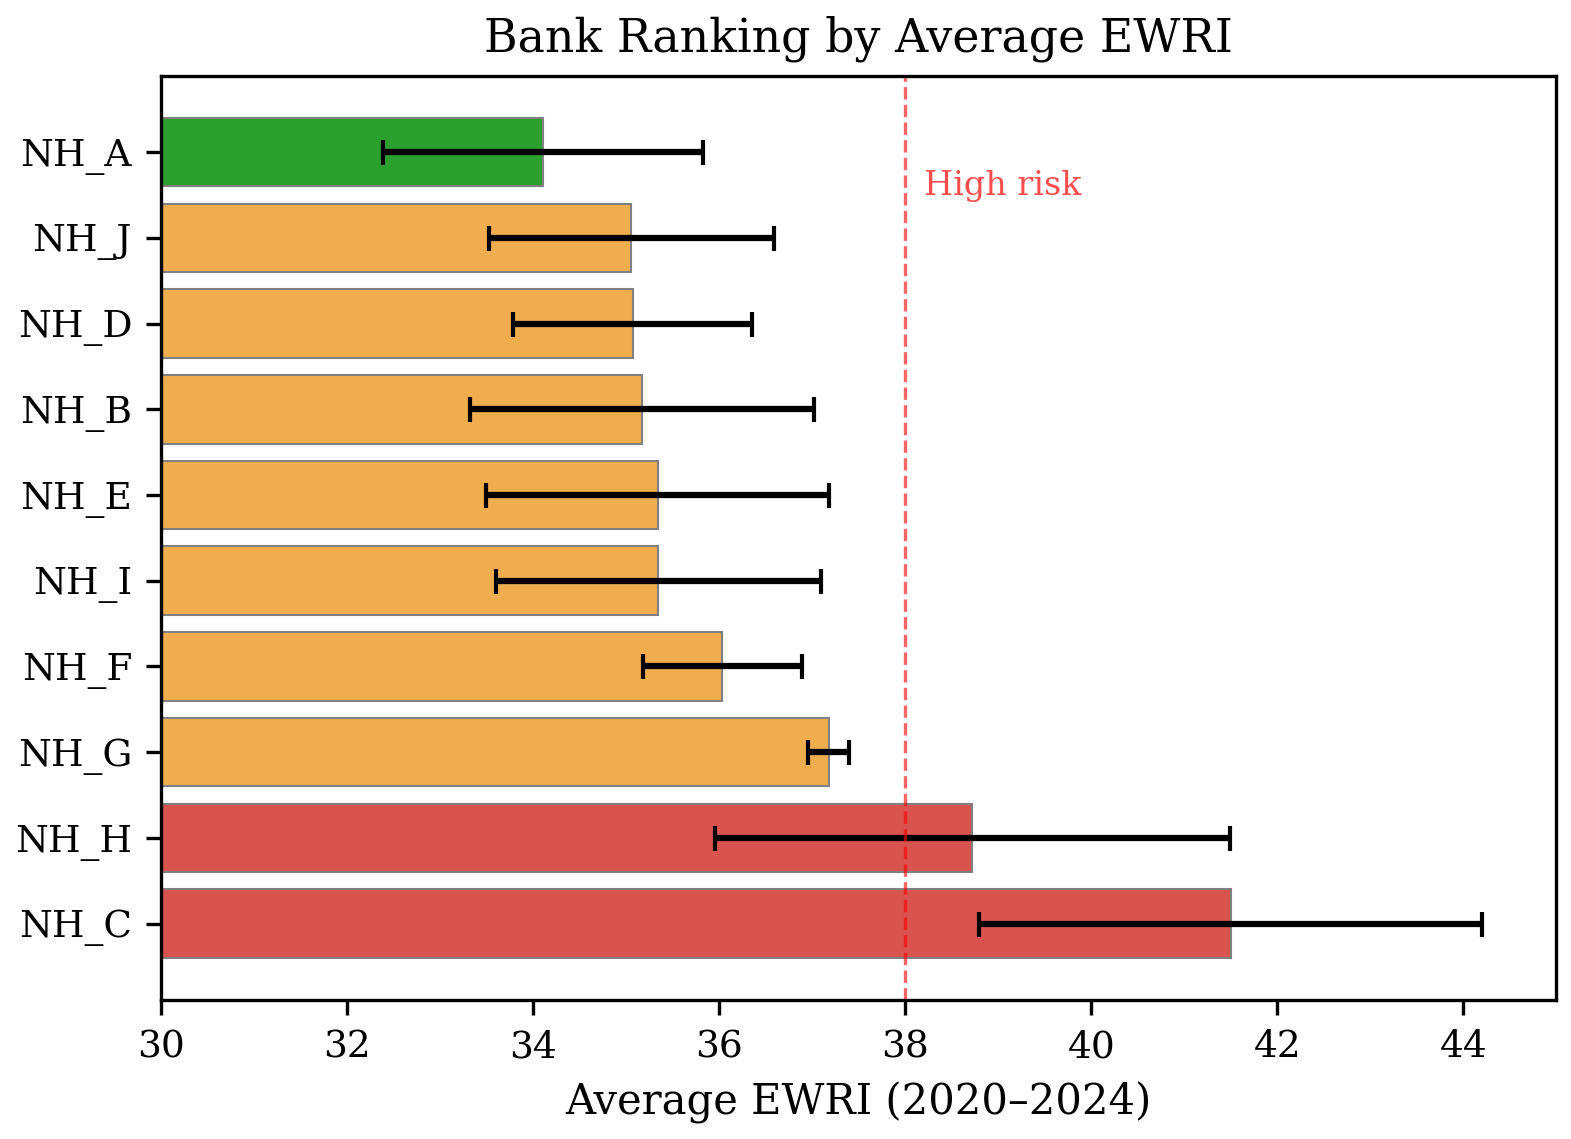
\includegraphics[width=0.75\textwidth]{figures/bank_ranking.png}
    \caption{Xếp hạng ngân hàng theo EWRI trung bình (2020--2024). Thanh lỗi thể hiện độ lệch chuẩn. Đường đỏ đứt nét: ngưỡng rủi ro High ($\geq 38$). Ngân hàng có EWRI thấp hơn được đánh giá minh bạch ESG tốt hơn.}
    \label{fig:bank_ranking}
\end{figure}

\begin{table}[H]
\centering
\caption{Chi tiết xếp hạng ngân hàng theo EWRI trung bình (2020--2024). $\bar{R}_I$: tỉ lệ Implemented; $\bar{R}_{In}$: tỉ lệ Indeterminate; $\bar{R}_E$: tỉ lệ có bằng chứng.}
\label{tab:bank_ranking_detail}
\small
\begin{tabular}{clcccccc}
\toprule
\textbf{Hạng} & \textbf{Ngân hàng} & \textbf{EWRI} & \textbf{Std} & \textbf{$\bar{R}_I$} & \textbf{$\bar{R}_{In}$} & \textbf{$\bar{R}_E$} & \textbf{Số câu} \\
\midrule
1  & NH\_A  & 34,10 & 1,72 & 36,8\% & 60,5\% & 30,1\% & 1.544 \\
2  & NH\_J  & 35,05 & 1,42 & 34,9\% & 62,3\% & 24,5\% & 3.398 \\
3  & NH\_D  & 35,07 & 1,67 & 33,7\% & 63,0\% & 25,0\% & 2.912 \\
4  & NH\_B  & 35,17 & 1,19 & 34,3\% & 62,2\% & 28,2\% & 5.138 \\
5  & NH\_E  & 35,34 & 2,33 & 34,4\% & 64,2\% & 26,6\% & 2.014 \\
6  & NH\_I  & 35,34 & 0,94 & 33,7\% & 64,2\% & 24,1\% & 5.022 \\
7  & NH\_F  & 36,03 & 2,04 & 32,8\% & 64,8\% & 25,6\% & 2.850 \\
8  & NH\_G  & 37,18 & 2,67 & 29,3\% & 66,9\% & 20,9\% & 3.754 \\
9  & NH\_H  & 38,72 & 3,42 & 27,4\% & 70,4\% & 16,5\% & 2.972 \\
10 & NH\_C  & 41,50 & 2,04 & 21,9\% & 76,7\% & 20,1\% & 2.656 \\
\bottomrule
\end{tabular}
\end{table}

NH\_A dẫn đầu với EWRI thấp nhất (34,10), nhờ tỉ lệ Implemented cao nhất (36,8\%) và tỉ lệ Indeterminate thấp nhất (60,5\%). NH\_C xếp cuối với EWRI = 41,50 --- duy nhất thuộc nhóm High risk trung bình (có một quan sát Very~High ở năm 2020 với EWRI = 45,75). NH\_H xếp hạng 9/10 do tỉ lệ Indeterminate cao (70,4\%) và tỉ lệ bằng chứng thấp nhất (16,5\%).

Khoảng cách giữa nhóm dẫn đầu (hạng 1--4, EWRI $\approx$ 34--35) và nhóm cuối (hạng 9--10, EWRI $\approx$ 39--42) là khoảng 7 điểm --- phân biệt có ý nghĩa với hệ số biến thiên CV = 7,4\% của công thức nhân.


\subsection{Bản đồ nhiệt EWRI}
\label{subsec:ewri_heatmap}

Hình~\ref{fig:ewri_heatmap} trực quan hóa EWRI cho tất cả 50 quan sát ngân hàng-năm dưới dạng bản đồ nhiệt. Các ô màu càng đỏ thể hiện rủi ro ESG-washing càng cao.

\begin{figure}[H]
    \centering
    
\includegraphics[width=0.8\textwidth]{figures/ewri_heatmap.png}
    \caption{Bản đồ nhiệt EWRI theo ngân hàng và năm (2020--2024). Ngân hàng được sắp xếp theo EWRI trung bình tăng dần. Màu xanh: rủi ro thấp; Màu đỏ: rủi ro cao.}
    \label{fig:ewri_heatmap}
\end{figure}


\subsection{Phân tích theo chủ đề ESG}
\label{subsec:topic_ewri}

Bảng~\ref{tab:topic_ewri} phân tích EWRI theo từng chủ đề, và Hình~\ref{fig:topic_distribution} trực quan hóa phân phối chủ đề ESG cùng tỉ lệ hành động theo từng chủ đề.

\begin{table}[H]
\centering
\caption{EWRI và phân phối hành động theo chủ đề ESG.}
\label{tab:topic_ewri}
\begin{tabular}{lrccccc}
\toprule
\textbf{Chủ đề} & \textbf{N} & \textbf{\%} & \textbf{EWRI} & \textbf{Impl\,\%} & \textbf{Plan\,\%} & \textbf{Indet\,\%} \\
\midrule
E              &  3.029 &  9,4 & 33,33 & 37,6 &  5,2 & 57,2 \\
S\_community   &  1.996 &  6,2 & 32,91 & 41,2 &  0,7 & 58,1 \\
S\_product     &  4.866 & 15,1 & 34,94 & 36,6 &  3,1 & 60,4 \\
S\_labor       &  5.584 & 17,3 & 36,42 & 33,1 &  1,7 & 65,2 \\
G              & 16.785 & 52,0 & 37,13 & 28,7 &  3,0 & 68,4 \\
\bottomrule
\end{tabular}
\end{table}

\begin{figure}[H]
    \centering
    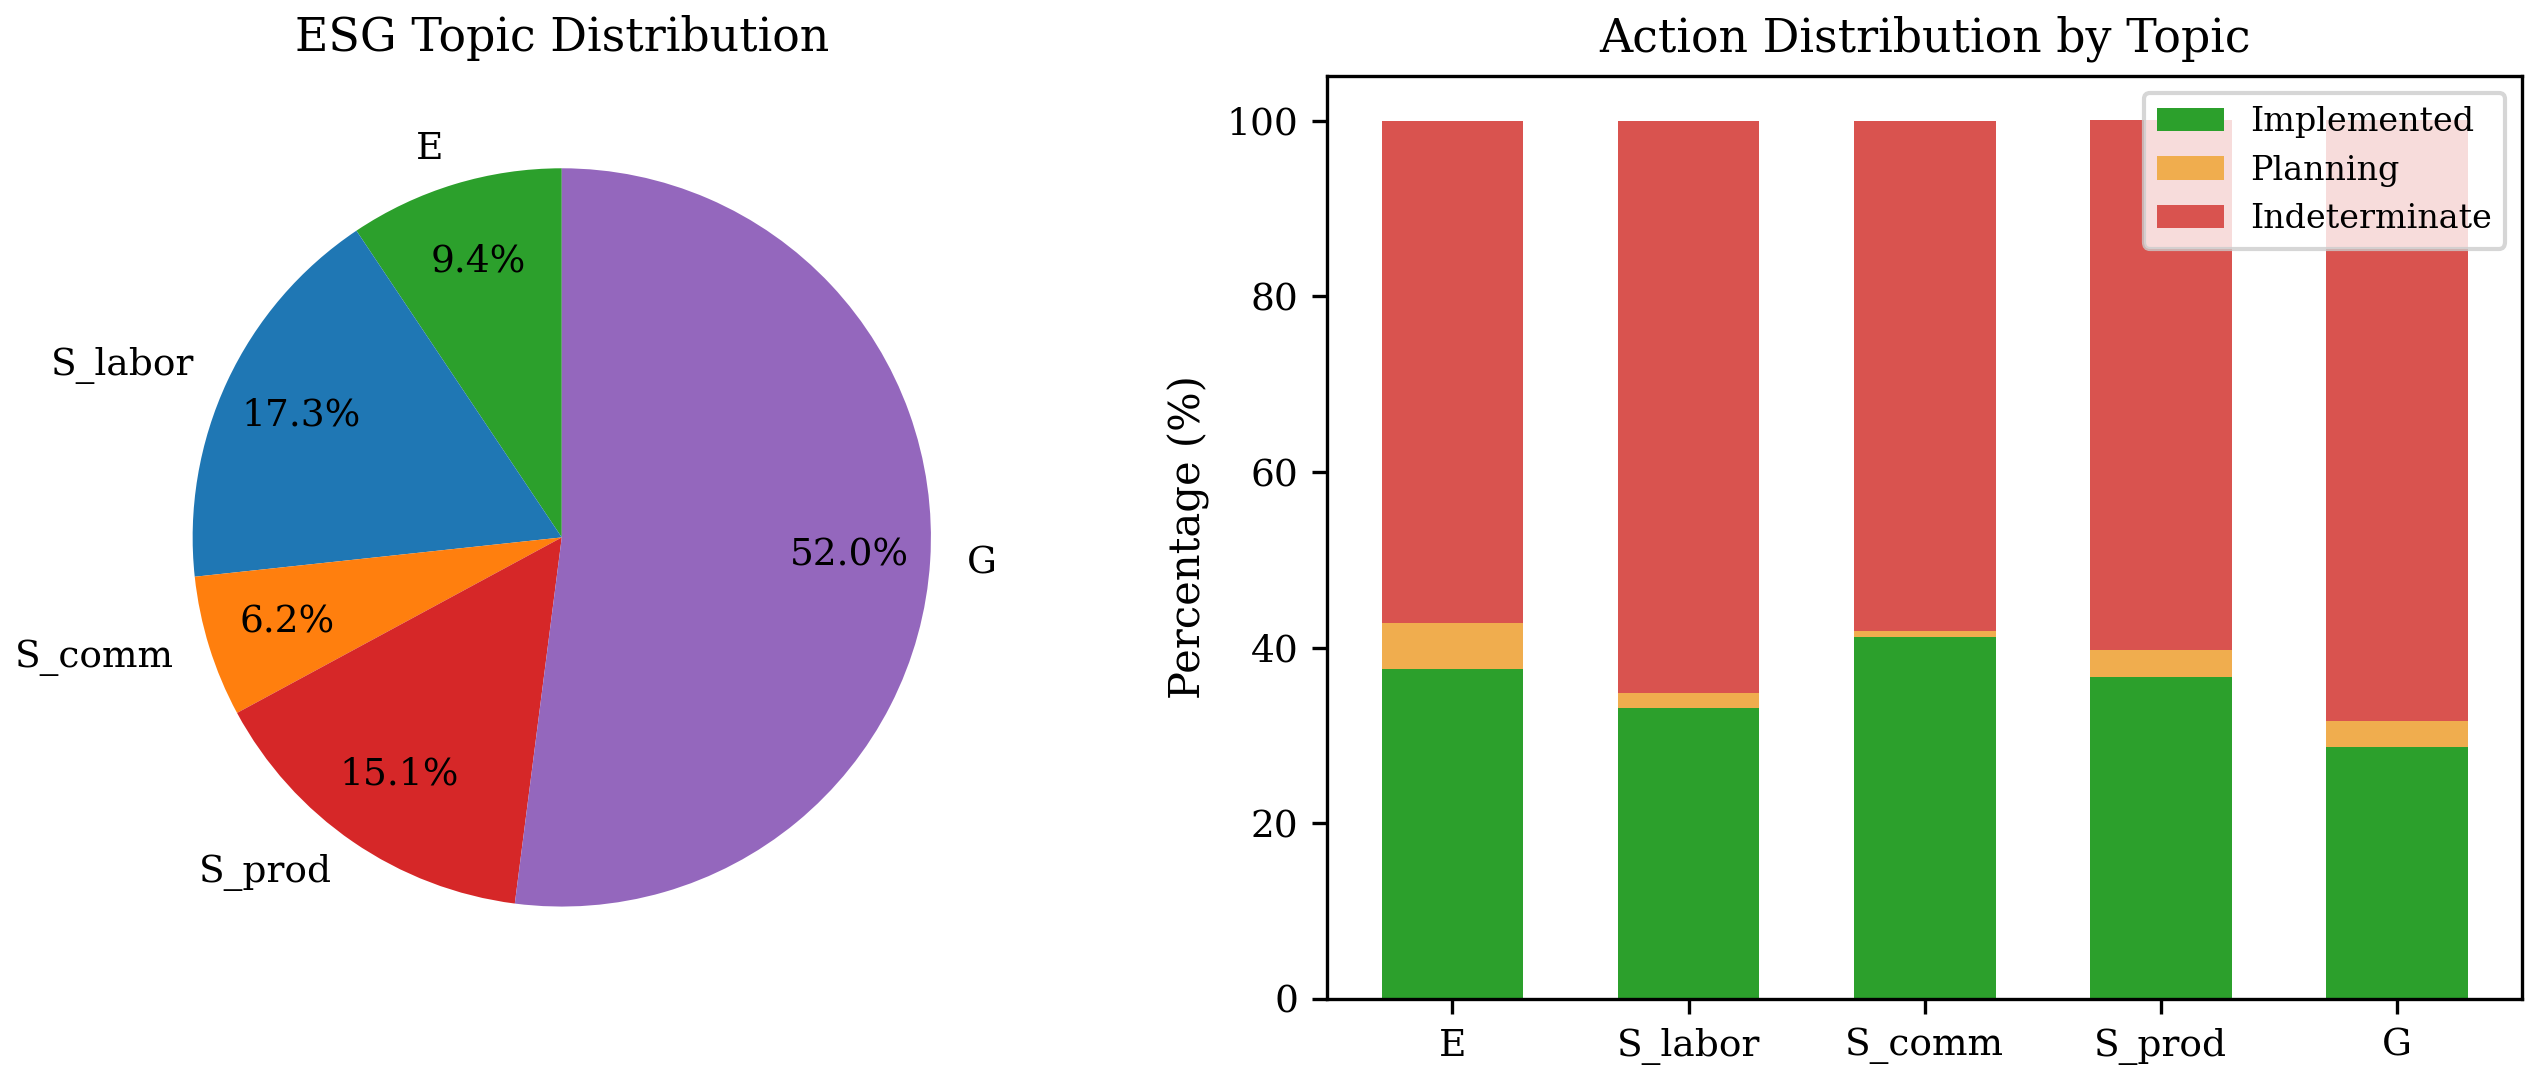
\includegraphics[width=0.95\textwidth]{figures/topic_distribution.png}
    \caption{Trái: Phân phối chủ đề ESG trong corpus (32.260 câu). Phải: Phân phối nhãn hành động theo từng chủ đề.}
    \label{fig:topic_distribution}
\end{figure}

Chủ đề G (Quản trị) chiếm tỉ trọng lớn nhất (52,0\%) và có EWRI cao nhất (37,13), phản ánh xu hướng các ngân hàng dành nhiều nội dung cho quản trị doanh nghiệp nhưng chủ yếu ở mức mơ hồ (68,4\% Indeterminate). Ngược lại, chủ đề S\_community (6,2\%) có EWRI thấp nhất (32,91) với tỉ lệ Implemented cao nhất (41,2\%) --- phù hợp với thực tế rằng các hoạt động cộng đồng thường có bằng chứng cụ thể hơn (ví dụ: số tiền quyên góp, số công trình xây dựng).

Chủ đề E (Môi trường) có tỉ lệ Planning cao nhất (5,2\%), cho thấy các ngân hàng có xu hướng đưa ra nhiều kế hoạch liên quan đến môi trường (cam kết giảm phát thải, lộ trình Net Zero) nhưng chưa có nhiều bằng chứng thực hiện.


\subsection{Vai trò các loại bằng chứng}
\label{subsec:evidence_type_importance}

Bảng~\ref{tab:evidence_types} và Hình~\ref{fig:evidence_types} phân tích mức độ giảm rủi ro khi có từng loại bằng chứng.

\begin{table}[H]
\centering
\caption{Tầm quan trọng của bốn loại bằng chứng. $\overline{\text{WRS}}_+$: washing risk trung bình khi có bằng chứng; $\overline{\text{WRS}}_-$: washing risk khi không có.}
\label{tab:evidence_types}
\begin{tabular}{lrccc}
\toprule
\textbf{Loại BC} & \textbf{Tần suất} & \textbf{$\overline{\text{WRS}}_+$} & \textbf{$\overline{\text{WRS}}_-$} & \textbf{Giảm rủi ro} \\
\midrule
KPI          & 2.231 (6,9\%) & 0,092 & 0,381 & 75,8\% \\
Time\_bound  & 3.663 (11,4\%) & 0,195 & 0,382 & 48,9\% \\
Standard     & 1.837 (5,7\%) & 0,273 & 0,366 & 25,3\% \\
Third\_party & 1.663 (5,2\%) & 0,298 & 0,364 & 18,3\% \\
\bottomrule
\end{tabular}
\end{table}

\begin{figure}[H]
    \centering
    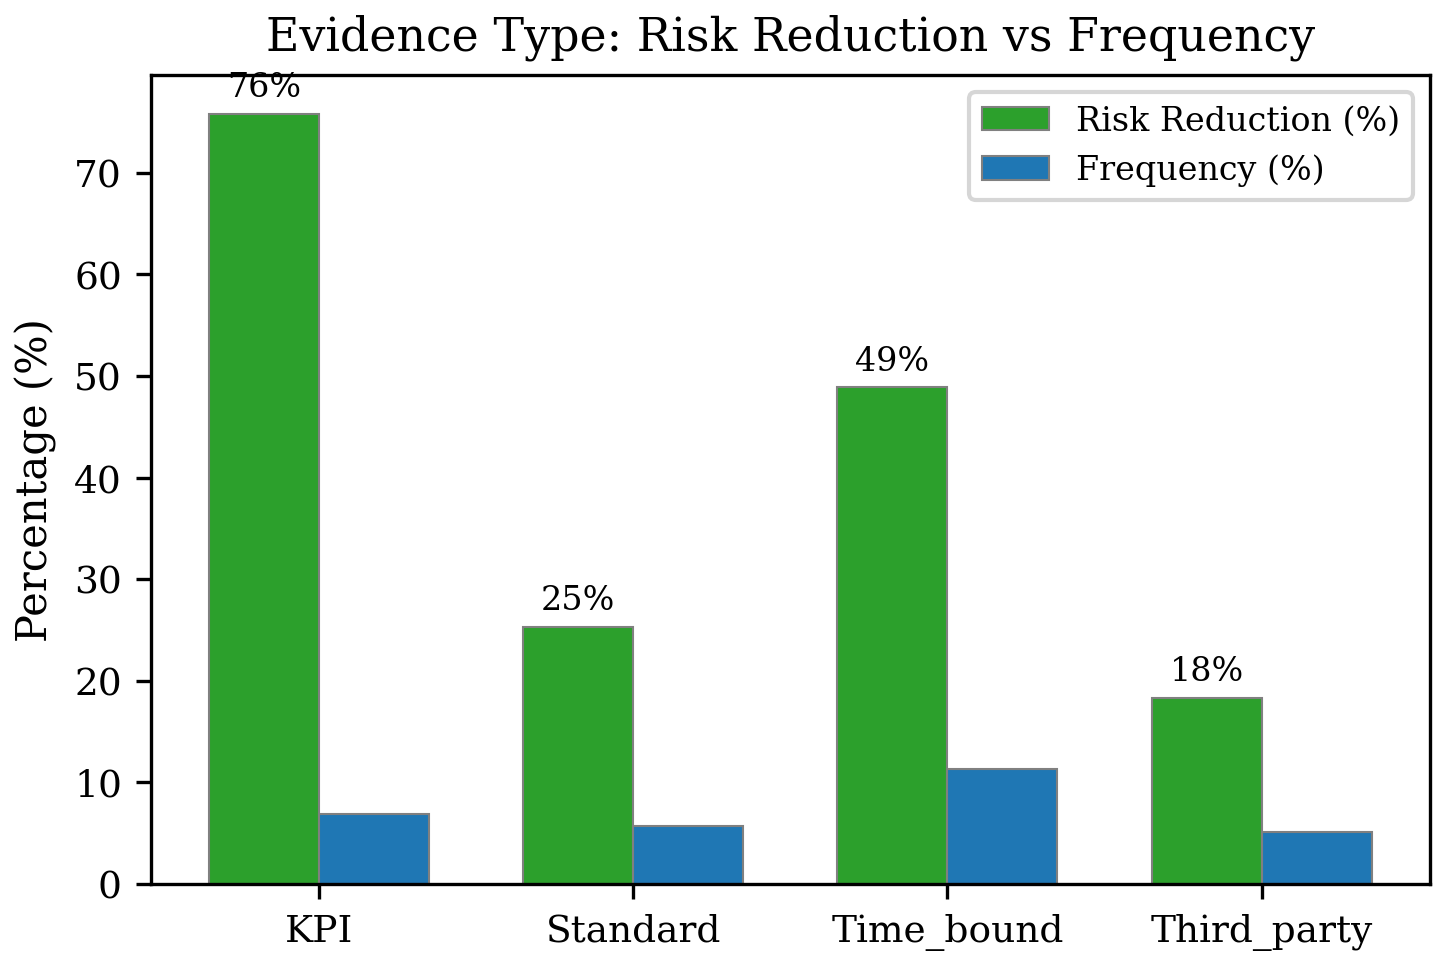
\includegraphics[width=0.65\textwidth]{figures/evidence_types.png}
    \caption{So sánh mức giảm rủi ro và tần suất xuất hiện của bốn loại bằng chứng.}
    \label{fig:evidence_types}
\end{figure}

Bằng chứng KPI (chỉ số đo lường cụ thể) cho hiệu quả giảm rủi ro cao nhất (75,8\%), đưa trung bình washing risk từ 0,381 xuống 0,092. Tuy nhiên, loại bằng chứng này chỉ xuất hiện ở 6,9\% câu ESG. Time\_bound (cam kết có mốc thời gian) xuất hiện phổ biến hơn (11,4\%) và giảm rủi ro 48,9\%. Hai loại Standard và Third\_party có hiệu quả giảm rủi ro thấp hơn (25,3\% và 18,3\%), phần nào do tính chất gián tiếp: viện dẫn tiêu chuẩn hay bên thứ ba giúp tăng độ tin cậy nhưng không trực tiếp chứng minh kết quả.


\subsection{Xu hướng thời gian (2020--2024)}
\label{subsec:temporal_trends}

Hình~\ref{fig:temporal_trends} và Bảng~\ref{tab:temporal} trình bày diễn biến EWRI trung bình qua 5 năm.

\begin{table}[H]
\centering
\caption{Xu hướng EWRI và các chỉ số hành động theo năm.}
\label{tab:temporal}
\begin{tabular}{cccccc}
\toprule
\textbf{Năm} & \textbf{EWRI} & \textbf{Std} & \textbf{Impl\,\%} & \textbf{Indet\,\%} & \textbf{BC\,\%} \\
\midrule
2020 & 37,08 & 4,13 & 30,8 & 66,5 & 23,6 \\
2021 & 35,67 & 2,93 & 34,0 & 63,9 & 26,9 \\
2022 & 35,98 & 1,79 & 32,6 & 65,0 & 26,1 \\
2023 & 36,13 & 2,13 & 32,1 & 65,6 & 24,1 \\
2024 & 36,90 & 2,08 & 30,2 & 66,6 & 24,0 \\
\bottomrule
\end{tabular}
\end{table}

\begin{figure}[H]
    \centering
    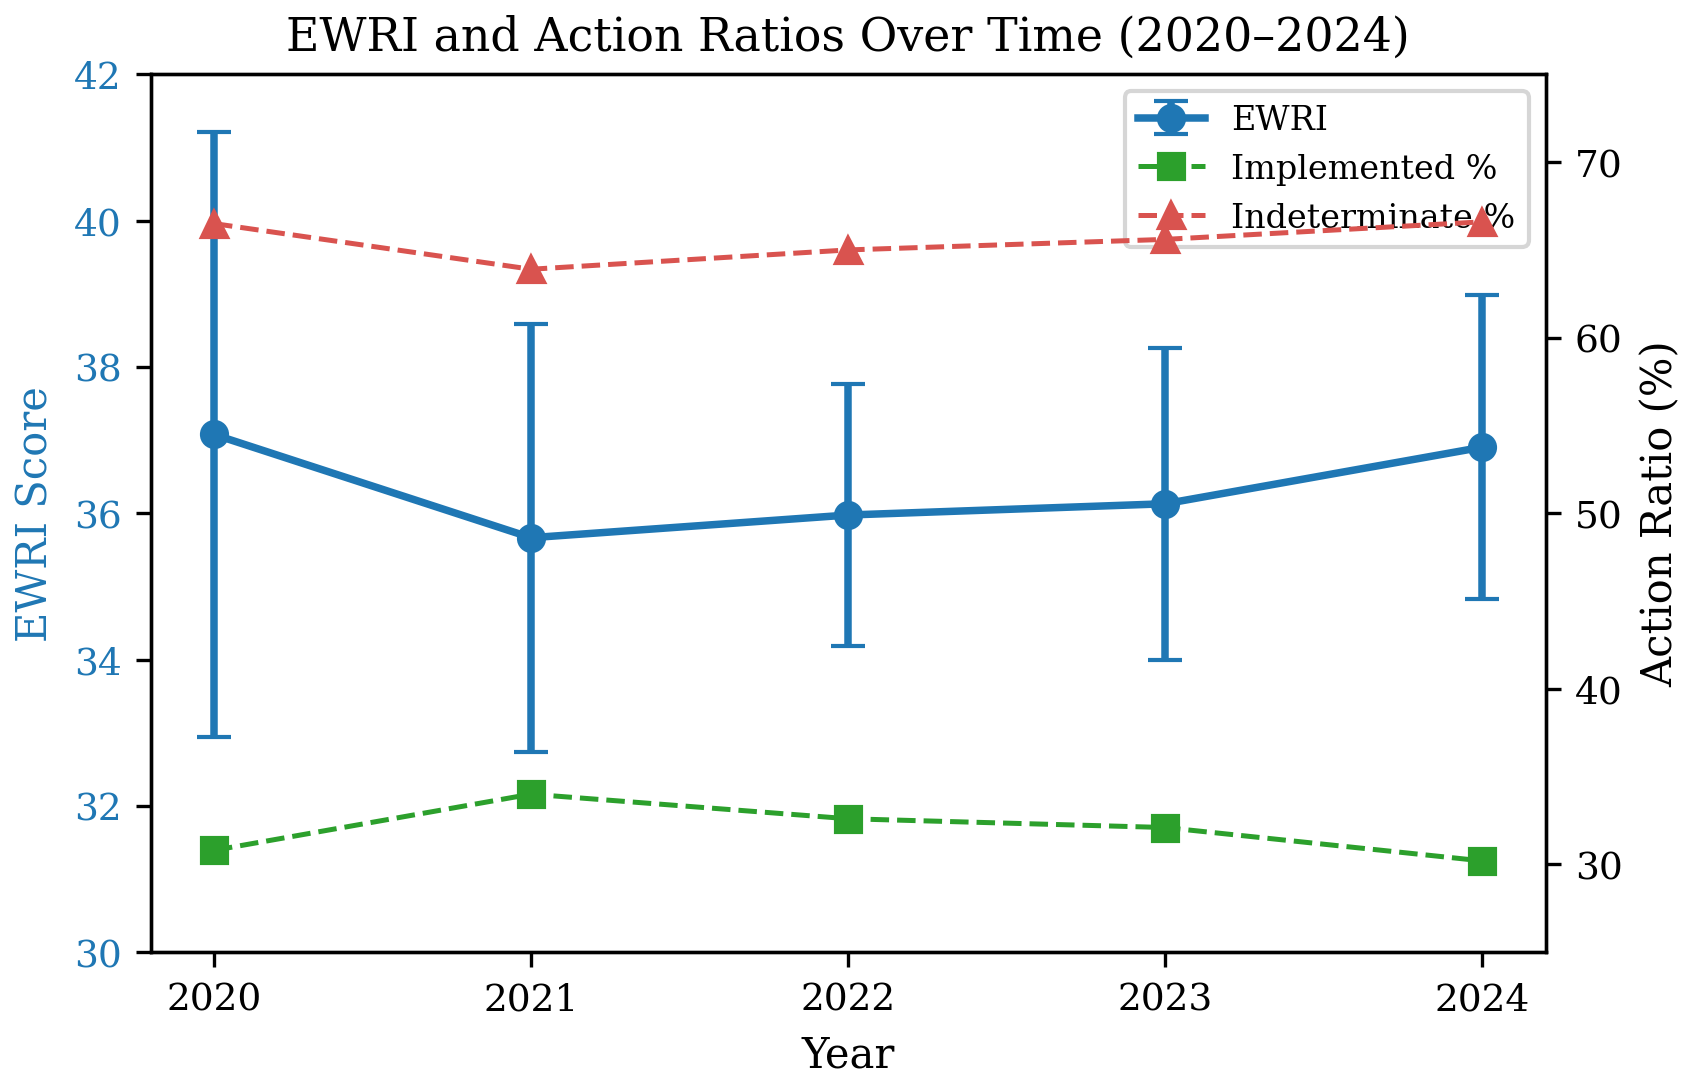
\includegraphics[width=0.75\textwidth]{figures/temporal_trends.png}
    \caption{Diễn biến EWRI và tỉ lệ hành động qua giai đoạn 2020--2024. Trục trái: EWRI (điểm, thấp hơn = minh bạch hơn); Trục phải: tỉ lệ Implemented và Indeterminate (\%).}
    \label{fig:temporal_trends}
\end{figure}

Xu hướng thời gian cho thấy mô hình \textit{U-shaped}: EWRI giảm từ 37,08 (2020) xuống 35,67 (2021) --- mức thấp nhất trong giai đoạn --- sau đó tăng dần lên 36,90 (2024). Năm 2021 ghi nhận tỉ lệ Implemented cao nhất (34,0\%) và tỉ lệ có bằng chứng cao nhất (26,9\%), có thể liên quan đến áp lực hậu COVID-19 buộc các ngân hàng báo cáo cụ thể hơn về các hành động đã thực hiện.

Từ 2022 trở đi, EWRI có xu hướng tăng nhẹ, đi kèm giảm tỉ lệ Implemented (từ 34,0\% xuống 30,2\%) và tăng tỉ lệ Indeterminate (từ 63,9\% lên 66,6\%). Xu hướng này gợi ý rằng dù khối lượng báo cáo ESG tăng (số câu ESG tăng), chất lượng cam kết không cải thiện tương ứng --- một biểu hiện có thể của \textit{ESG-washing leo thang} (escalating greenwashing), nhất quán với phát hiện của \citet{marquis2016scrutiny} về hiện tượng ``selective disclosure'' ở các thị trường mới nổi.

Đáng lưu ý, độ lệch chuẩn giảm mạnh từ 4,13 (2020) xuống 1,79 (2022), cho thấy sự hội tụ trong chất lượng báo cáo ESG giữa các ngân hàng --- có thể do ảnh hưởng của các hướng dẫn quy chuẩn (như GRI Standards) bắt đầu được áp dụng rộng rãi hơn.


\subsection{So sánh công thức tính EWRI}
\label{subsec:formula_comparison}

Để đánh giá hiệu quả của công thức nhân (multiplicative) đề xuất so với công thức cộng (additive) đơn giản, khóa luận tính EWRI theo cả hai công thức trên cùng tập dữ liệu.

\begin{table}[H]
\centering
\caption{So sánh công thức cộng (additive) và công thức nhân (multiplicative) trên 50 quan sát.}
\label{tab:formula_comparison}
\begin{tabular}{lcc}
\toprule
\textbf{Chỉ số} & \textbf{Additive} & \textbf{Multiplicative} \\
\midrule
Trung bình ($\mu$)      & 54,32 & 36,35 \\
Độ lệch chuẩn ($\sigma$) & 2,85 & 2,69 \\
Hệ số biến thiên (CV)    & 5,3\% & 7,4\% \\
Phạm vi (Range)           & 13,01 & 14,07 \\
Tương quan hạng (Spearman) & \multicolumn{2}{c}{$\rho = 0{,}998$} \\
\bottomrule
\end{tabular}
\end{table}

\begin{figure}[H]
    \centering
    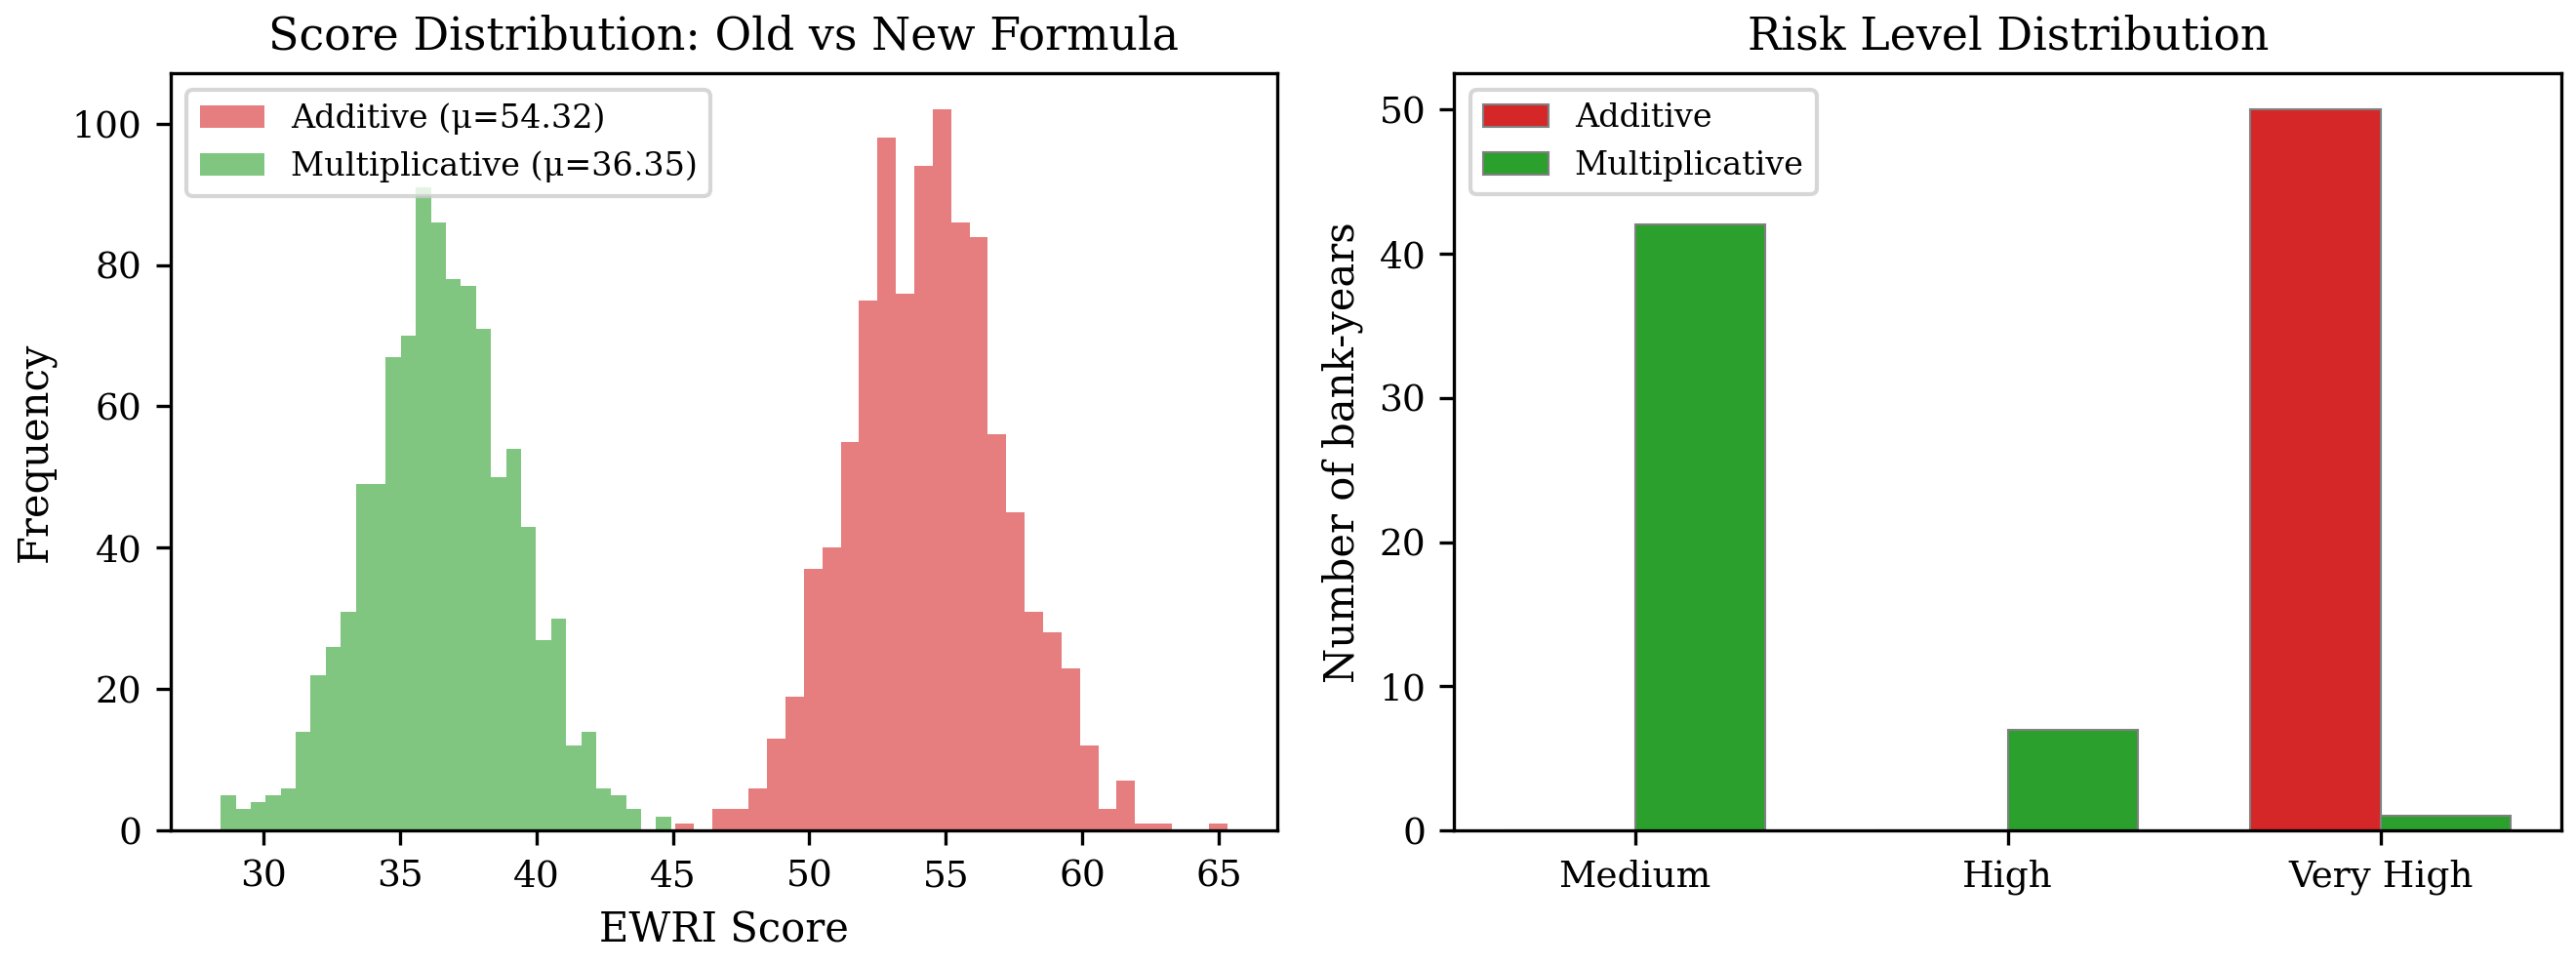
\includegraphics[width=0.95\textwidth]{figures/formula_comparison.png}
    \caption{So sánh hai công thức EWRI. Trái: phân phối điểm (mô phỏng); Phải: phân phối mức rủi ro.}
    \label{fig:formula_comparison}
\end{figure}

Hai công thức có tương quan hạng rất cao ($\rho = 0{,}998$), nghĩa là thứ hạng các ngân hàng gần như không thay đổi. Tuy nhiên, công thức nhân mang lại hai cải thiện quan trọng: (1) Hệ số biến thiên CV tăng từ 5,3\% lên 7,4\%, cho phép phân biệt tốt hơn giữa các ngân hàng; (2) Phân phối mức rủi ro hợp lý hơn --- thay vì tất cả 50 quan sát cùng xếp vào Very~High, công thức nhân phân phối thành 42 Medium, 7 High, và 1 Very~High, phản ánh chính xác hơn sự đa dạng trong chất lượng báo cáo ESG.


\subsection{Phân tích tương quan}
\label{subsec:correlation_analysis}

Hình~\ref{fig:correlation_heatmap} trình bày ma trận tương quan Spearman giữa các biến EWRI.

\begin{figure}[H]
    \centering
    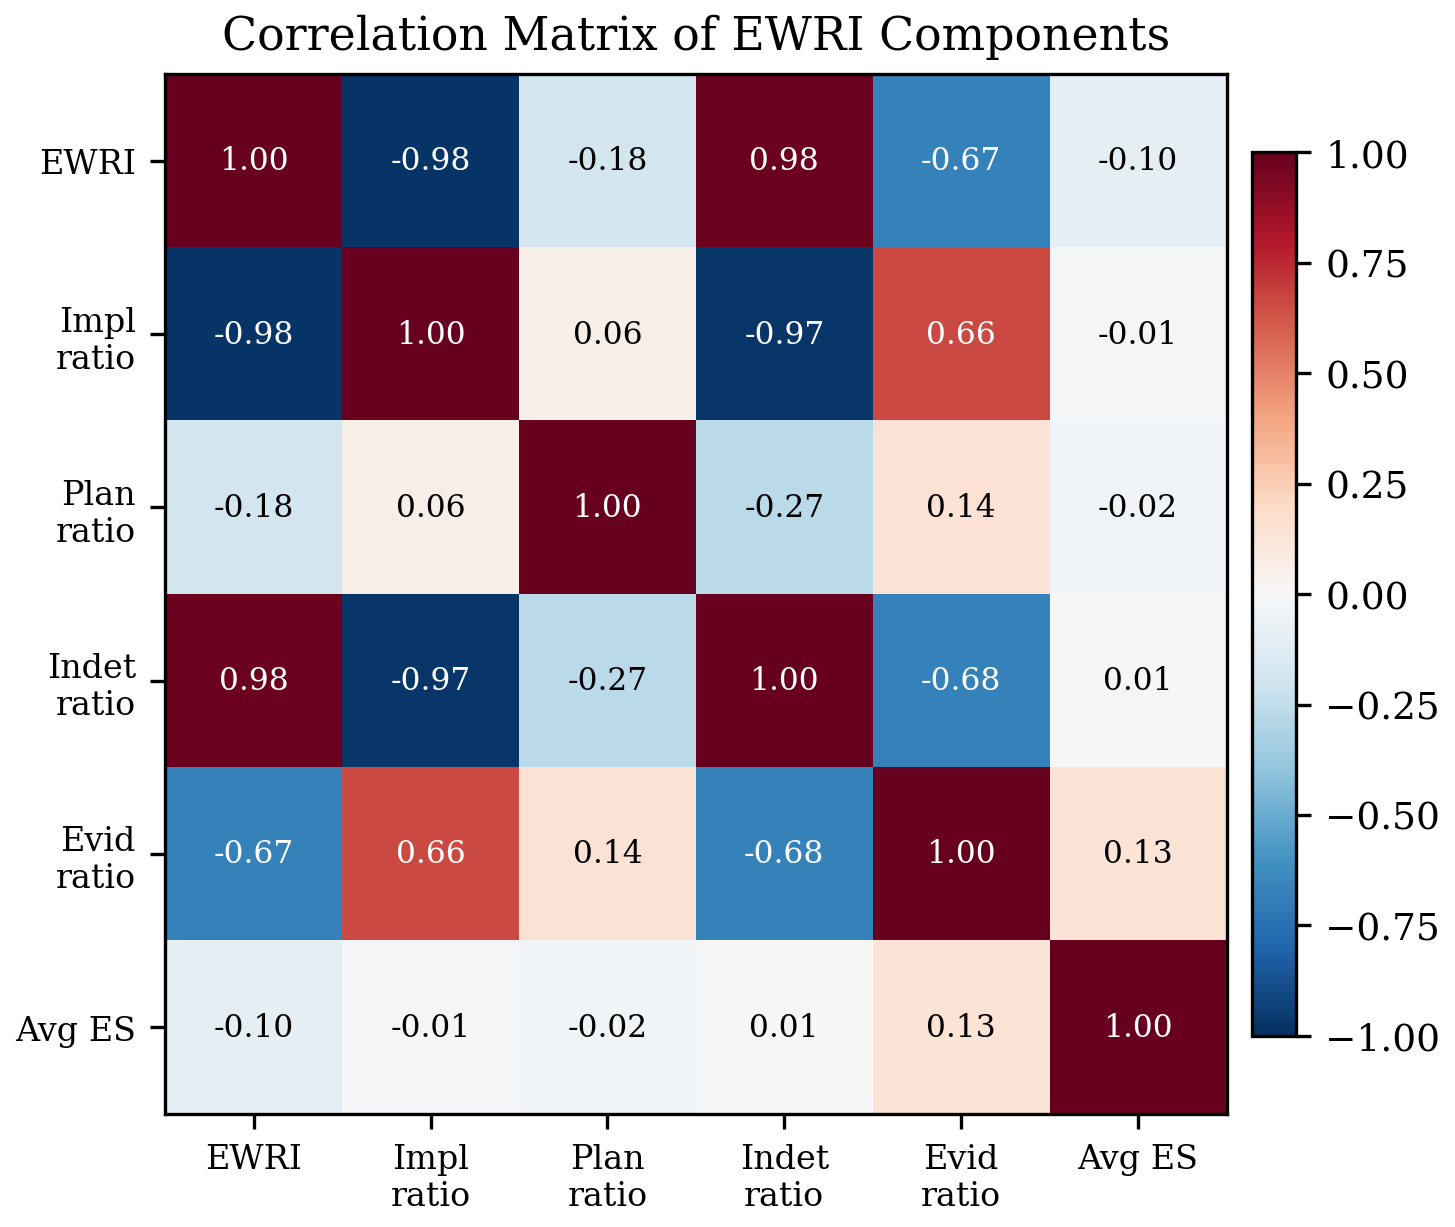
\includegraphics[width=0.6\textwidth]{figures/correlation_heatmap.png}
    \caption{Ma trận tương quan Spearman giữa EWRI và các thành phần. Màu đỏ: tương quan dương; Màu xanh: tương quan âm.}
    \label{fig:correlation_heatmap}
\end{figure}

Các nhận định chính từ phân tích tương quan:

\begin{itemize}
    \item EWRI tương quan dương rất mạnh với tỉ lệ Indeterminate ($\rho = 0{,}983$, $p < 0{,}001$) và tương quan âm rất mạnh với tỉ lệ Implemented ($\rho = -0{,}977$, $p < 0{,}001$). Điều này xác nhận rằng nhãn hành động --- đặc biệt là sự phân biệt giữa cam kết đã thực hiện và cam kết mơ hồ --- là yếu tố quyết định chính của EWRI.
    \item Tỉ lệ bằng chứng (evidence ratio) có tương quan âm vừa phải với EWRI ($\rho = -0{,}672$), nghĩa là bằng chứng đóng vai trò điều chỉnh nhưng không chi phối.
    \item Phân tích ANOVA cho thấy nhãn hành động giải thích 95,17\% phương sai của washing risk score ở mức câu ($\eta^2 = 0{,}952$), xác nhận vai trò chủ đạo của thành phần hành động trong công thức EWRI.
\end{itemize}


\subsection{Tổng hợp kết quả RQ3}
\label{subsec:rq3_answer}

\begin{tcolorbox}[colback=gray!5, colframe=gray!60, title=Trả lời RQ3]
Chỉ số EWRI phản ánh phù hợp mức độ rủi ro ESG-washing trên 50 quan sát ngân hàng-năm. Kết quả cho thấy: (1) Phân biệt rõ ràng giữa 10 ngân hàng, với khoảng cách EWRI trung bình 7,4 điểm giữa nhóm tốt nhất (NH\_A, 34,10) và kém nhất (NH\_C, 41,50); (2) Xu hướng thời gian dạng U-shaped: cải thiện năm 2021 sau đó quay lại mức cũ, cho thấy không có tiến bộ bền vững về minh bạch ESG; (3) Công thức nhân (multiplicative) vượt trội công thức cộng với CV tăng 40\% (7,4\% so với 5,3\%) trong khi giữ nguyên thứ hạng ($\rho = 0{,}998$).
\end{tcolorbox}


%% ============================================================
%% 4.7 PHÂN TÍCH ĐỊNH TÍNH
%% ============================================================
\section{Phân tích định tính}
\label{sec:qualitative}

Để minh họa khả năng giải thích (interpretability) của hệ thống và chứng minh pipeline hoạt động đúng, phần này phân tích chi tiết các trường hợp cụ thể cùng bảng ví dụ đại diện với nội dung câu thực tế.

\subsection{Trường hợp rủi ro cao (High-risk ESG-washing)}
\label{subsec:high_risk_case}

\begin{quote}
\textit{``...chính sách và 02 chương trình mục tiêu quốc gia, xây dựng các sản phẩm tín dụng ưu đãi phù hợp với nhiều đối tượng khách hàng, phát triển đa dạng các dịch vụ, kênh phân phối hỗ trợ người dân và doanh nghiệp...''} \\
--- NH\_A, 2023 \quad $\bullet$ Chủ đề: S\_product \quad $\bullet$ Hành động: Indeterminate \quad $\bullet$ ES = 0,000 \quad $\bullet$ WRS = 0,715
\end{quote}

Câu này được hệ thống đánh giá rủi ro cao nhất (WRS = 0,715) vì: (1) nhãn hành động là Indeterminate --- câu đề cập đến ``chính sách'' và ``chương trình mục tiêu'' nhưng không nêu rõ đã thực hiện hay mới chỉ là kế hoạch; (2) không có bằng chứng đi kèm (ES = 0); (3) thiếu KPI, mốc thời gian, hay tham chiếu bên thứ ba. Đây là ví dụ điển hình của ESG-washing: sử dụng ngôn ngữ mơ hồ để tạo ấn tượng tích cực mà không cung cấp thông tin kiểm chứng.

\subsection{Trường hợp rủi ro thấp (Substantive ESG reporting)}
\label{subsec:low_risk_case}

\begin{quote}
\textit{``Tỷ trọng tín dụng xanh tại Ngân hàng [NH\_F] hiện đã lên tới hơn 10\% trên tổng danh mục cho vay, phát huy hiệu quả rõ rệt, góp phần tăng trưởng bền vững và bảo vệ môi trường.''} \\
\textbf{Bằng chứng liên kết:} \textit{``Tỷ trọng tín dụng xanh tại Ngân hàng [NH\_F] hiện đã lên tới hơn 10\% trên tổng danh mục cho vay, phát huy hiệu quả rõ rệt góp phần tăng trưởng bền vững và bảo vệ môi trường.''} \\
--- NH\_F, 2023 \quad $\bullet$ Chủ đề: E \quad $\bullet$ Hành động: Implemented \quad $\bullet$ ES = 0,734 \quad $\bullet$ WRS = 0,033 \\
$\bullet$ Loại BC: KPI \quad $\bullet$ NLI: \textit{entailment}
\end{quote}

Câu này được đánh giá rủi ro rất thấp (WRS = 0,033) nhờ ba yếu tố cùng tác động: (1) nhãn hành động là Implemented --- ``đã lên tới hơn 10\%'' cho thấy kết quả đã đạt được; (2) bằng chứng mạnh (ES = 0,734) với KPI cụ thể (``hơn 10\% trên tổng danh mục cho vay''); (3) NLI xác nhận \textit{entailment} --- câu bằng chứng thực sự hỗ trợ tuyên bố. Đây là ví dụ của báo cáo ESG thực chất.


\subsection{Ví dụ đại diện toàn pipeline}
\label{subsec:representative_examples}

Bảng~\ref{tab:qual_examples} trình bày năm ví dụ đại diện từ các mức rủi ro và chủ đề khác nhau, bao gồm nội dung tuyên bố, bằng chứng liên kết, và các điểm số do hệ thống gán. Mỗi ví dụ minh họa một khía cạnh khác nhau của pipeline.

\begin{table}[H]
\centering
\caption{Năm ví dụ đại diện minh họa hoạt động pipeline. TBố: tuyên bố; BC: bằng chứng liên kết.}
\label{tab:qual_examples}
\footnotesize
\begin{tabular}{p{0.38\textwidth}p{0.15\textwidth}p{0.12\textwidth}p{0.07\textwidth}p{0.07\textwidth}p{0.07\textwidth}}
\toprule
\textbf{Nội dung (rút gọn)} & \textbf{Chủ đề / Hành động} & \textbf{Loại BC} & \textbf{NLI} & \textbf{ES} & \textbf{WRS} \\
\midrule
\textit{TBố:} ``...chính sách và 02 chương trình mục tiêu quốc gia, xây dựng các sản phẩm tín dụng ưu đãi...'' \newline \textit{BC:} Không có
    & S\_product / Indeterminate & --- & --- & 0,000 & 0,715 \\
\midrule
\textit{TBố:} ``Chúng tôi sẽ tăng cường hợp tác với các đối tác quốc tế để thu hút nguồn vốn xanh, tích hợp các tiêu chuẩn ESG chặt chẽ hơn...'' \newline \textit{BC:} ``...nỗ lực này góp phần cải thiện môi trường sống...''
    & E / Planning & --- & neutral & 0,000 & 0,300 \\
\midrule
\textit{TBố:} ``96\% số lượng nhân viên có trình độ trên đại học đảm bảo nền tảng kiến thức chuyên môn...'' \newline \textit{BC:} \textit{(câu tương tự trong ngữ cảnh khác)}
    & S\_labor / Implemented & KPI & entail. & 0,737 & 0,033 \\
\midrule
\textit{TBố:} ``[NH\_F] đã hoàn tất 03 trụ cột của Hiệp ước vốn Basel II từ năm 2020 và tiếp tục triển khai theo phương pháp nâng cao...'' \newline \textit{BC:} ``[NH\_F] cũng đã hoàn tất 03 trụ cột Basel II từ năm 2020, đáp ứng tuân thủ toàn diện...''
    & G / Implemented & Std, Time & entail. & 0,762 & 0,031 \\
\midrule
\textit{TBố:} ``Tỷ trọng tín dụng xanh tại Ngân hàng [NH\_F] hiện đã lên tới hơn 10\% trên tổng danh mục cho vay...'' \newline \textit{BC:} \textit{(câu tương tự xác nhận)}
    & E / Implemented & KPI & entail. & 0,734 & 0,033 \\
\bottomrule
\end{tabular}
\end{table}

Các ví dụ trên cho thấy pipeline hoạt động đúng qua ba khía cạnh: (1) \textit{Phân loại hành động}: hệ thống phân biệt chính xác giữa ngôn ngữ mơ hồ (``chính sách'', ``chương trình mục tiêu'' $\to$ Indeterminate), ngôn ngữ kế hoạch (``sẽ tăng cường'' $\to$ Planning), và ngôn ngữ đã thực hiện (``đã hoàn tất'', ``đã lên tới'' $\to$ Implemented). (2) \textit{Liên kết bằng chứng}: hệ thống tìm được bằng chứng tương đồng ngữ nghĩa từ ngữ cảnh tài liệu; câu Implemented có bằng chứng mạnh (ES $>$ 0,7), trong khi câu Indeterminate/Planning thiếu bằng chứng (ES = 0). (3) \textit{NLI verification}: mô hình NLI xác nhận \textit{entailment} cho các cặp tuyên bố-bằng chứng thực sự hỗ trợ nhau (ví dụ: ``đã hoàn tất 03 trụ cột Basel II'' và bằng chứng xác nhận cùng nội dung), trong khi đánh giá \textit{neutral} cho các cặp có liên quan chủ đề nhưng không trực tiếp xác nhận.


\subsection{Kiểm tra chất lượng}
\label{subsec:quality_check}

Hệ thống thực hiện kiểm tra chất lượng (quality check) trên 100 câu có washing risk cao nhất: tỉ lệ nhiễu (noise rate) là 0,0\%, nghĩa là tất cả 100 câu đều là tuyên bố ESG thực sự (không phải lỗi phân loại chủ đề). Kết quả này xác nhận rằng bộ phân loại chủ đề ESG hoạt động đáng tin cậy trên các câu có rủi ro cao --- nhóm câu quan trọng nhất cho mục đích phát hiện ESG-washing.


%% ============================================================
%% 4.8 THẢO LUẬN
%% ============================================================
\section{Thảo luận}
\label{sec:discussion}

\subsection{Tổng hợp kết quả}
\label{subsec:results_summary}

Bảng~\ref{tab:results_summary} tổng hợp kết quả chính của toàn bộ pipeline.

\begin{table}[H]
\centering
\caption{Tổng hợp kết quả chính của hệ thống phát hiện ESG-washing.}
\label{tab:results_summary}
\small
\begin{tabular}{p{4.5cm}p{8cm}}
\toprule
\textbf{Thành phần} & \textbf{Kết quả chính} \\
\midrule
Phân loại chủ đề (6 nhãn)
    & Macro F1 = 0,83; Micro F1 = 0,91. Neuro $\approx$ Baseline (+0,4\% topic, +6,4\% action). \\
Phân loại hành động (3 nhãn)
    & Macro F1 = 0,78 (Neuro); Micro F1 = 0,89. Neuro vượt trội Baseline. \\
Liên kết bằng chứng
    & 24,6\% câu có BC; NLI loại 2,93\% mâu thuẫn; Semantic > Window (+11,8\% sim). \\
EWRI (50 ngân hàng-năm)
    & $\mu = 36{,}35 \pm 2{,}69$; 42 Medium / 7 High / 1 Very High; CV = 7,4\%. \\
\bottomrule
\end{tabular}
\end{table}


\subsection{Điểm mạnh}
\label{subsec:strengths}

Hệ thống đề xuất có một số điểm mạnh nổi bật. Thứ nhất, tính \textit{tự khép kín}: toàn bộ phân tích chỉ sử dụng dữ liệu nội tại trong báo cáo, không phụ thuộc nguồn ESG bên ngoài --- phù hợp với bối cảnh thị trường Việt Nam nơi hạ tầng giám sát ESG còn non trẻ. Thứ hai, \textit{khả năng giải thích}: mỗi điểm rủi ro đều có thể truy vết về câu cụ thể, nhãn hành động, loại bằng chứng và kết quả NLI --- cho phép người dùng hiểu tại sao một tuyên bố bị đánh giá rủi ro cao. Thứ ba, \textit{tính tổng quát}: cách tiếp cận neuro-symbolic kết hợp tri thức miền ESG có thể mở rộng sang các ngành khác (bất động sản, năng lượng) hoặc ngôn ngữ khác bằng cách thay đổi bộ quy tắc ký hiệu và mô hình ngôn ngữ nền tảng.


\subsection{Hạn chế}
\label{subsec:limitations}

Khóa luận nhận diện một số hạn chế cần được lưu ý. Thứ nhất, \textit{dữ liệu nhãn} được tạo bằng phương pháp chắt lọc từ LLM (Gemini 1.5 Flash) với đối chiếu quy tắc ký hiệu, nhưng chưa có gold-standard do chuyên gia gán thủ công, vì vậy chưa thể đánh giá trực tiếp chất lượng nhãn huấn luyện. Thứ hai, \textit{quy mô dữ liệu} (10 ngân hàng, 5 năm) tuy đủ để rút ra những kết luận ban đầu nhưng chưa đại diện cho toàn bộ hệ thống ngân hàng Việt Nam (hiện có hơn 30 ngân hàng thương mại). Thứ ba, \textit{tỉ lệ bằng chứng thấp} (24,6\%) có thể phản ánh giới hạn xử lý văn bản hơn là thực tế báo cáo --- một số bằng chứng ở dạng bảng biểu, hình ảnh, hoặc phụ lục mà pipeline hiện tại chưa xử lý được. Thứ tư, khóa luận chưa thực hiện đánh giá so sánh trực tiếp với các phương pháp phát hiện greenwashing khác (ví dụ phương pháp dựa trên NLP truyền thống hoặc thang đo thủ công) do hạn chế về thời gian và không có baseline công khai trên dữ liệu tiếng Việt.


\subsection{Đề xuất cải tiến}
\label{subsec:future_work}

Dựa trên các hạn chế trên, khóa luận đề xuất một số hướng cải tiến: (1) Xây dựng tập đánh giá gold-standard với sự tham gia của chuyên gia ESG và kiểm toán viên; (2) Mở rộng corpus sang các ngành khác (bất động sản, năng lượng, sản xuất) và tăng số lượng ngân hàng; (3) Tích hợp xử lý bảng biểu và hình ảnh bằng multimodal models để tăng tỉ lệ bằng chứng; (4) Thử nghiệm các mô hình ngôn ngữ lớn hơn (PhoBERT-large, ViDeBERTa) và kiến trúc multi-task learning cho hai bài toán phân loại đồng thời; (5) Áp dụng cross-validation hoặc multiple random seeds để đánh giá ổn định hơn.

